\section{Empirical results}\label{empirical-results}

\subsection{Behavioural estimates}\label{behavioural-estimates}

The estimated model has 41 free coordinates for single adults, of which 40 are interior, and 47 for couples, all interior. The criterion is 6253.463 and 10283.034 respectively. Across ten terminal paths from five starts under two polishing contracts, the criterion varies by 1.1e-10 for single adults and 1.3e-09 for couples, and the smallest eigenvalue of the exact Hessian on the interior block is 0.1669 and 0.0771. One single-adult coordinate, the female age-square term in the leisure weight, sits at a box endpoint; its interval is reported under the active-set convention in the appendix and it is excluded from the interior curvature.

\Needspace*{12\baselineskip}\small\setlength{\tabcolsep}{3pt}\begin{longtable}[]{@{}
  >{\raggedright\arraybackslash}p{(\linewidth - 8\tabcolsep) * \real{0.2000}}
  >{\raggedright\arraybackslash}p{(\linewidth - 8\tabcolsep) * \real{0.2000}}
  >{\raggedright\arraybackslash}p{(\linewidth - 8\tabcolsep) * \real{0.2000}}
  >{\raggedright\arraybackslash}p{(\linewidth - 8\tabcolsep) * \real{0.2000}}
  >{\raggedright\arraybackslash}p{(\linewidth - 8\tabcolsep) * \real{0.2000}}@{}}
\caption{The preference block. Cluster-robust standard errors in parentheses, clustered on the household. ``At bound'' marks an estimate at a box endpoint, whose interval is reported under the active-set convention in the appendix. The consumption weight is common within a population and enters as \(\beta_c\log(C/\lambda_c)\).}\tabularnewline
\toprule\noalign{}
\begin{minipage}[b]{\linewidth}\raggedright
Coefficient
\end{minipage} & \begin{minipage}[b]{\linewidth}\raggedright
Single men
\end{minipage} & \begin{minipage}[b]{\linewidth}\raggedright
Single women
\end{minipage} & \begin{minipage}[b]{\linewidth}\raggedright
Couple men
\end{minipage} & \begin{minipage}[b]{\linewidth}\raggedright
Couple women
\end{minipage} \\
\midrule\noalign{}
\endfirsthead
\toprule\noalign{}
\begin{minipage}[b]{\linewidth}\raggedright
Coefficient
\end{minipage} & \begin{minipage}[b]{\linewidth}\raggedright
Single men
\end{minipage} & \begin{minipage}[b]{\linewidth}\raggedright
Single women
\end{minipage} & \begin{minipage}[b]{\linewidth}\raggedright
Couple men
\end{minipage} & \begin{minipage}[b]{\linewidth}\raggedright
Couple women
\end{minipage} \\
\midrule\noalign{}
\endhead
\bottomrule\noalign{}
\endlastfoot
Leisure weight, intercept \(\beta_{\ell 0}\) & 8.5199 (3.5480) & 5.8683 (2.1346) & 3.9814 (0.7466) & 13.1029 (4.7760) \\
Leisure weight, age \(\beta_{\ell a}\) & 1.4820 (1.0236) & 0.0678 (0.4792) & -0.0080 (0.0287) & -0.1228 (0.1260) \\
Leisure weight, age squared \(\beta_{\ell a^2}\) & 0.7783 (0.7732) & 1.0000 (at bound) & 0.0065 (0.0030) & 0.0073 (0.0103) \\
Leisure weight, children \(\beta_{\ell n}\) & --- & 0.1666 (0.4422) & --- & -0.3055 (1.1472) \\
Leisure curvature \(\theta_\ell\) & -1.6263 (0.3301) & -0.9274 (0.2161) & -0.9761 (0.1357) & -1.6863 (0.2458) \\
Consumption weight \(\beta_c\) & 2.0387 (0.2917) & 2.0387 (0.2917) & 2.1017 (0.2939) & 2.1017 (0.2939) \\
\end{longtable}

The consumption weight is 2.0387 with a cluster-robust standard error of 0.2917 for single adults and 2.1017 with 0.2939 for couples. Two things follow. Because the estimate exceeds one, the money metric of Section 4 is a power mean of order above one rather than an arithmetic mean. And because utility is on the unit-scale shock, one natural unit of the index corresponds to multiplying consumption by \(\exp(1/\beta_c)\), a factor of 1.633 for single adults and 1.609 for couples. That is a proportional statement: there is no single euro value of a unit of utility independent of the consumption at which it is evaluated.

\Needspace*{12\baselineskip}\small\setlength{\tabcolsep}{3pt}\begin{longtable}[]{@{}
  >{\raggedright\arraybackslash}p{(\linewidth - 6\tabcolsep) * \real{0.2500}}
  >{\raggedright\arraybackslash}p{(\linewidth - 6\tabcolsep) * \real{0.2500}}
  >{\raggedright\arraybackslash}p{(\linewidth - 6\tabcolsep) * \real{0.2500}}
  >{\raggedright\arraybackslash}p{(\linewidth - 6\tabcolsep) * \real{0.2500}}@{}}
\caption{The opportunity block: employment access, the hours density and occupation access. Cluster-robust standard errors in parentheses. The employment index multiplies the working indicator; the omitted references are region 1, thinly populated areas, the residual hours set of total width 26.5 hours per week, and occupation group 1. The singles occupation column reports the female coordinates; the male coordinates are in the appendix table. Hours coefficients are common across the two singles sex groups and spouse-specific for couples.}\tabularnewline
\toprule\noalign{}
\begin{minipage}[b]{\linewidth}\raggedright
Coefficient
\end{minipage} & \begin{minipage}[b]{\linewidth}\raggedright
Singles
\end{minipage} & \begin{minipage}[b]{\linewidth}\raggedright
Couple men
\end{minipage} & \begin{minipage}[b]{\linewidth}\raggedright
Couple women
\end{minipage} \\
\midrule\noalign{}
\endfirsthead
\toprule\noalign{}
\begin{minipage}[b]{\linewidth}\raggedright
Coefficient
\end{minipage} & \begin{minipage}[b]{\linewidth}\raggedright
Singles
\end{minipage} & \begin{minipage}[b]{\linewidth}\raggedright
Couple men
\end{minipage} & \begin{minipage}[b]{\linewidth}\raggedright
Couple women
\end{minipage} \\
\midrule\noalign{}
\endhead
\bottomrule\noalign{}
\endlastfoot
Employment constant \(\beta_E\) & -3.1735 (0.4053) & -2.1233 (0.3195) & -2.8148 (0.3021) \\
Group unemployment rate \(\beta_{E,gsur}\) & -1.4422 (0.2356) & -1.1924 (0.1557) & shared with the man \\
Densely populated \(\beta_{E,u}\) & -0.0288 (0.2209) & -0.1823 (0.1657) & shared with the man \\
Intermediate density \(\beta_{E,m}\) & 0.0641 (0.2614) & -0.4174 (0.1861) & shared with the man \\
Region 2 \(\beta_{E,2}\) & -0.3780 (0.3292) & -0.1546 (0.2442) & shared with the man \\
Region 3 \(\beta_{E,3}\) & -0.1117 (0.3891) & 0.0873 (0.2808) & shared with the man \\
Region 4 \(\beta_{E,4}\) & -0.8218 (0.3810) & 0.0150 (0.3068) & shared with the man \\
Region 5 \(\beta_{E,5}\) & -0.5162 (0.3274) & -0.1455 (0.2555) & shared with the man \\
Region 6 \(\beta_{E,6}\) & -0.7222 (0.3528) & -0.2844 (0.2748) & shared with the man \\
Region 7 \(\beta_{E,7}\) & -0.5374 (0.3503) & -0.1396 (0.2651) & shared with the man \\
Region 8 \(\beta_{E,8}\) & -0.4512 (0.3401) & -0.1659 (0.2660) & shared with the man \\
Hours band: Part-time lower, {[}17.5, 21.5) & 0.0298 (0.1972) & -1.1094 (0.3791) & -0.5173 (0.1629) \\
Hours band: Part-time upper, {[}28.5, 30.5) & 0.7080 (0.1928) & 0.0835 (0.2378) & 1.1586 (0.1214) \\
Hours band: Narrow full-time, {[}33.5, 36.5) & 2.0656 (0.0894) & 2.2888 (0.0821) & 2.0284 (0.0682) \\
Hours band: Full-time upper, {[}36.5, 40.5{]} & 1.9387 (0.0997) & 2.3801 (0.0866) & 1.6825 (0.0798) \\
Hours band: Long hours, {[}44.5, 70{]} & -0.0834 (0.1772) & 0.6977 (0.1335) & -0.3109 (0.1615) \\
Occupation 2 \(\xi_2\) & 0.1135 (0.1374) & -1.5097 (0.0967) & 0.2074 (0.0891) \\
Occupation 3 \(\xi_3\) & -0.4060 (0.1440) & -2.2532 (0.1244) & -0.1804 (0.0923) \\
Occupation 4 \(\xi_4\) & 0.5632 (0.1225) & 0.1594 (0.0618) & 0.8159 (0.0799) \\
\end{longtable}

\Needspace*{12\baselineskip}\small\setlength{\tabcolsep}{3pt}\begin{longtable}[]{@{}>{\RaggedRight\arraybackslash}p{0.4200\linewidth}>{\RaggedRight\arraybackslash}p{0.2590\linewidth}>{\RaggedRight\arraybackslash}p{0.2590\linewidth}@{}}
\caption{The wage block and the consumption weight. The offered log wage is normal with mean \(\mu_i(k)\) and dispersion \(\sigma\), truncated to {[}2, 590{]} EUR/hour and renormalized on that support. Experience enters in units of twenty years. Slopes and \(\sigma\) are common across the two singles sex groups and across spouses within couples; the singles and couples models are estimated separately, so the two columns are not restricted to agree.}\tabularnewline
\toprule\noalign{}
Coefficient & Singles & Couples \\
\midrule\noalign{}
\endfirsthead
\toprule\noalign{}
Coefficient & Singles & Couples \\
\midrule\noalign{}
\endhead
\bottomrule\noalign{}
\endlastfoot
Intercept \(\beta_{w0}\) & 2.0138 (0.0561) & 2.0480 (0.0335) \\
Low education \(\beta_{wL}\) & 0.0566 (0.0372) & -0.0433 (0.0217) \\
High education \(\beta_{wH}\) & 0.1491 (0.0308) & 0.1817 (0.0197) \\
Potential experience \(\beta_{wx}\) & 0.2408 (0.0862) & 0.5643 (0.0546) \\
Experience squared \(\beta_{wx^2}\) & -0.0282 (0.0390) & -0.1598 (0.0243) \\
Occupation 2 \(\delta_2\) & -0.0347 (0.0399) & -0.0740 (0.0231) \\
Occupation 3 \(\delta_3\) & 0.0622 (0.0383) & 0.0394 (0.0228) \\
Occupation 4 \(\delta_4\) & 0.2785 (0.0368) & 0.2146 (0.0223) \\
Log-wage dispersion \(\sigma\) & 0.3815 (0.0133) & 0.3631 (0.0072) \\
Consumption weight \(\beta_c\) & 2.0387 (0.2917) & 2.1017 (0.2939) \\
\end{longtable}

\textbf{Maintained restrictions.} Singles: \texttt{theta\_c\_singles\ =\ 0}; the couples preference block (\texttt{beta\_l0\_m}, \texttt{beta\_l\_age\_m}, \texttt{beta\_l\_age2\_m}, \texttt{beta\_l0\_f}, \texttt{beta\_l\_age\_f}, \texttt{beta\_l\_age2\_f}, \texttt{beta\_l\_nkids\_f}, \texttt{theta\_l\_f}) does not enter the singles likelihood; and \texttt{beta\_E\_y2015} and \texttt{beta\_E\_y2017} are absent because the 2015 and 2017 data are not used. Couples: \texttt{theta\_c\ =\ 0}, the male children leisure effect is structurally zero, and the direct cross-leisure term is fixed at zero. These are restrictions, not estimates. The singles and couples models are estimated separately, so their wage blocks are not restricted to agree, and the difference between the two experience profiles should not be read as a test.

\begin{figure}[H]
\centering
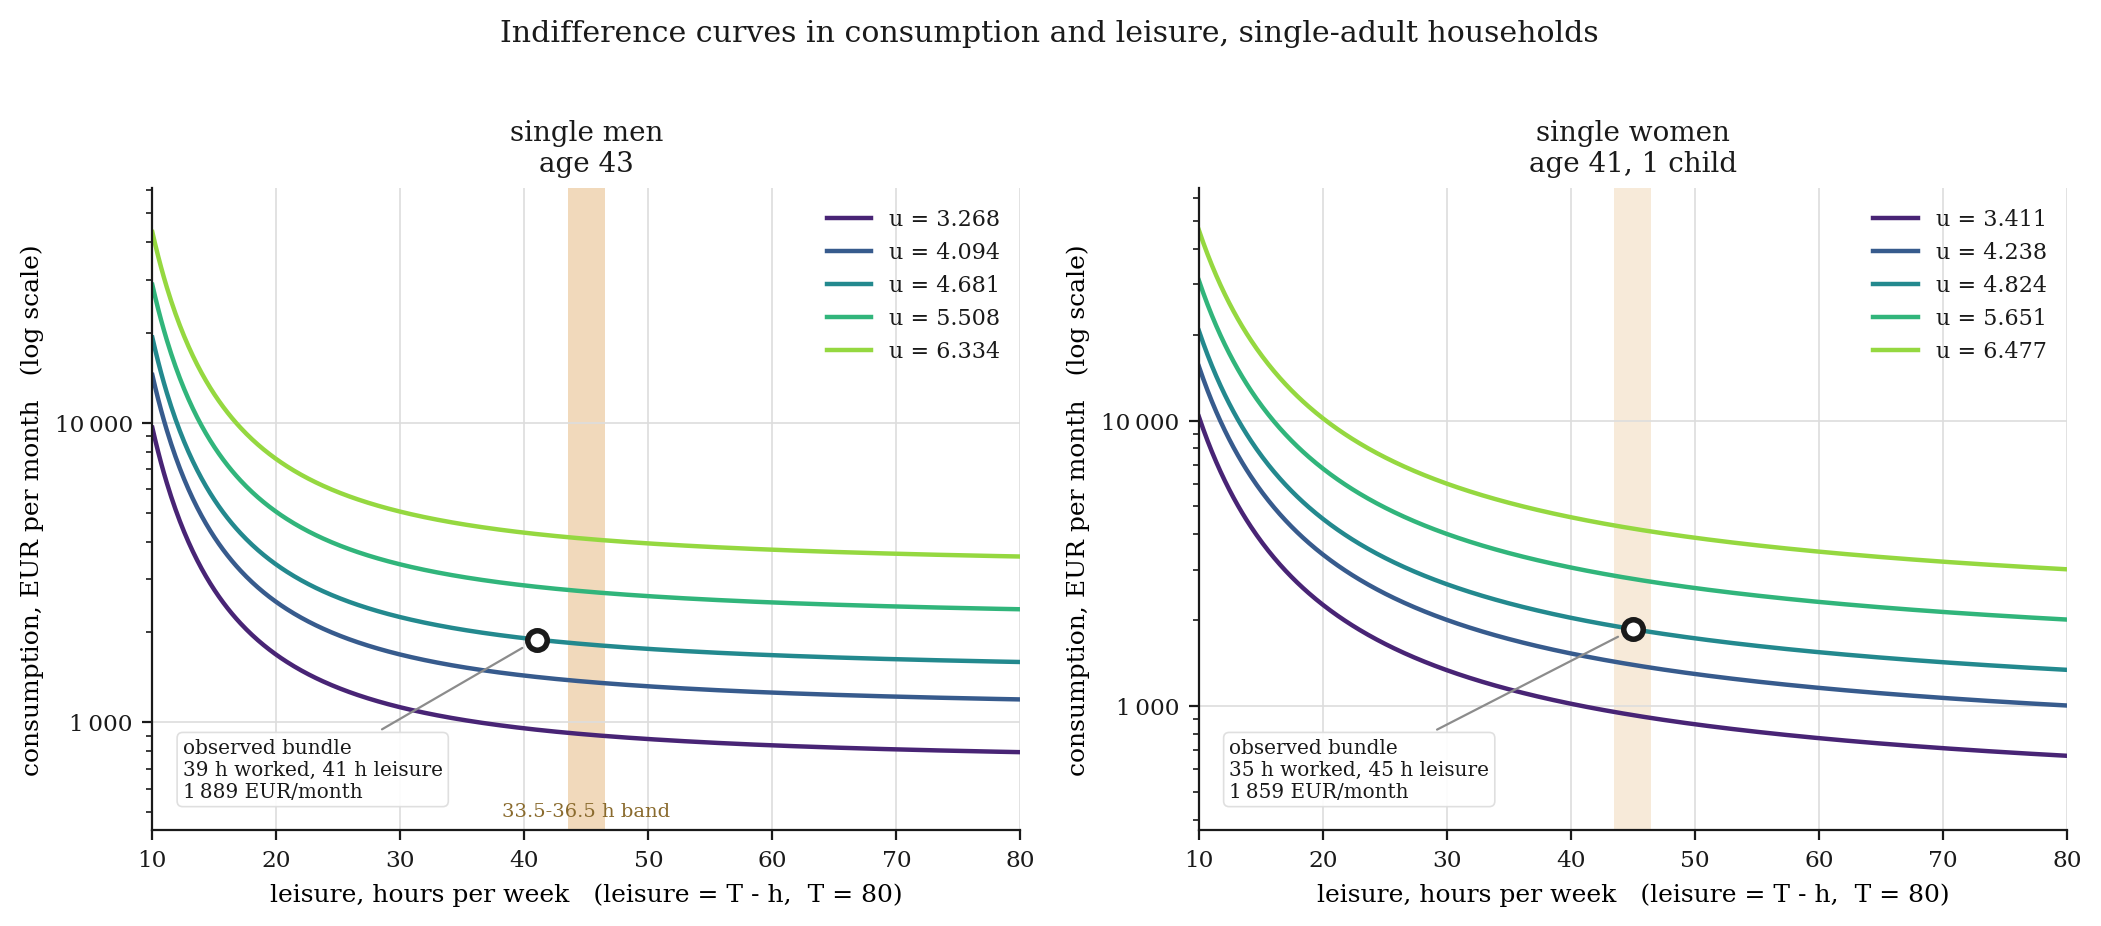
\includegraphics[width=0.95\linewidth,height=\textheight,keepaspectratio,alt={Indifference curves in consumption and leisure, single-adult households, at one representative household of each sex. The budget set, the opportunity density and the taste shock are not drawn, so a curve is not a set of attainable bundles. The consumption axis is logarithmic; under log consumption every finite utility target is attainable at a finite positive consumption, which may lie outside the plotted range.}]{figures/v5/figP01_indifference_curves_singles.png}
\caption{Indifference curves in consumption and leisure, single-adult households, at one representative household of each sex. The budget set, the opportunity density and the taste shock are not drawn, so a curve is not a set of attainable bundles. The consumption axis is logarithmic; under log consumption every finite utility target is attainable at a finite positive consumption, which may lie outside the plotted range.}
\end{figure}

\begin{figure}[H]
\centering
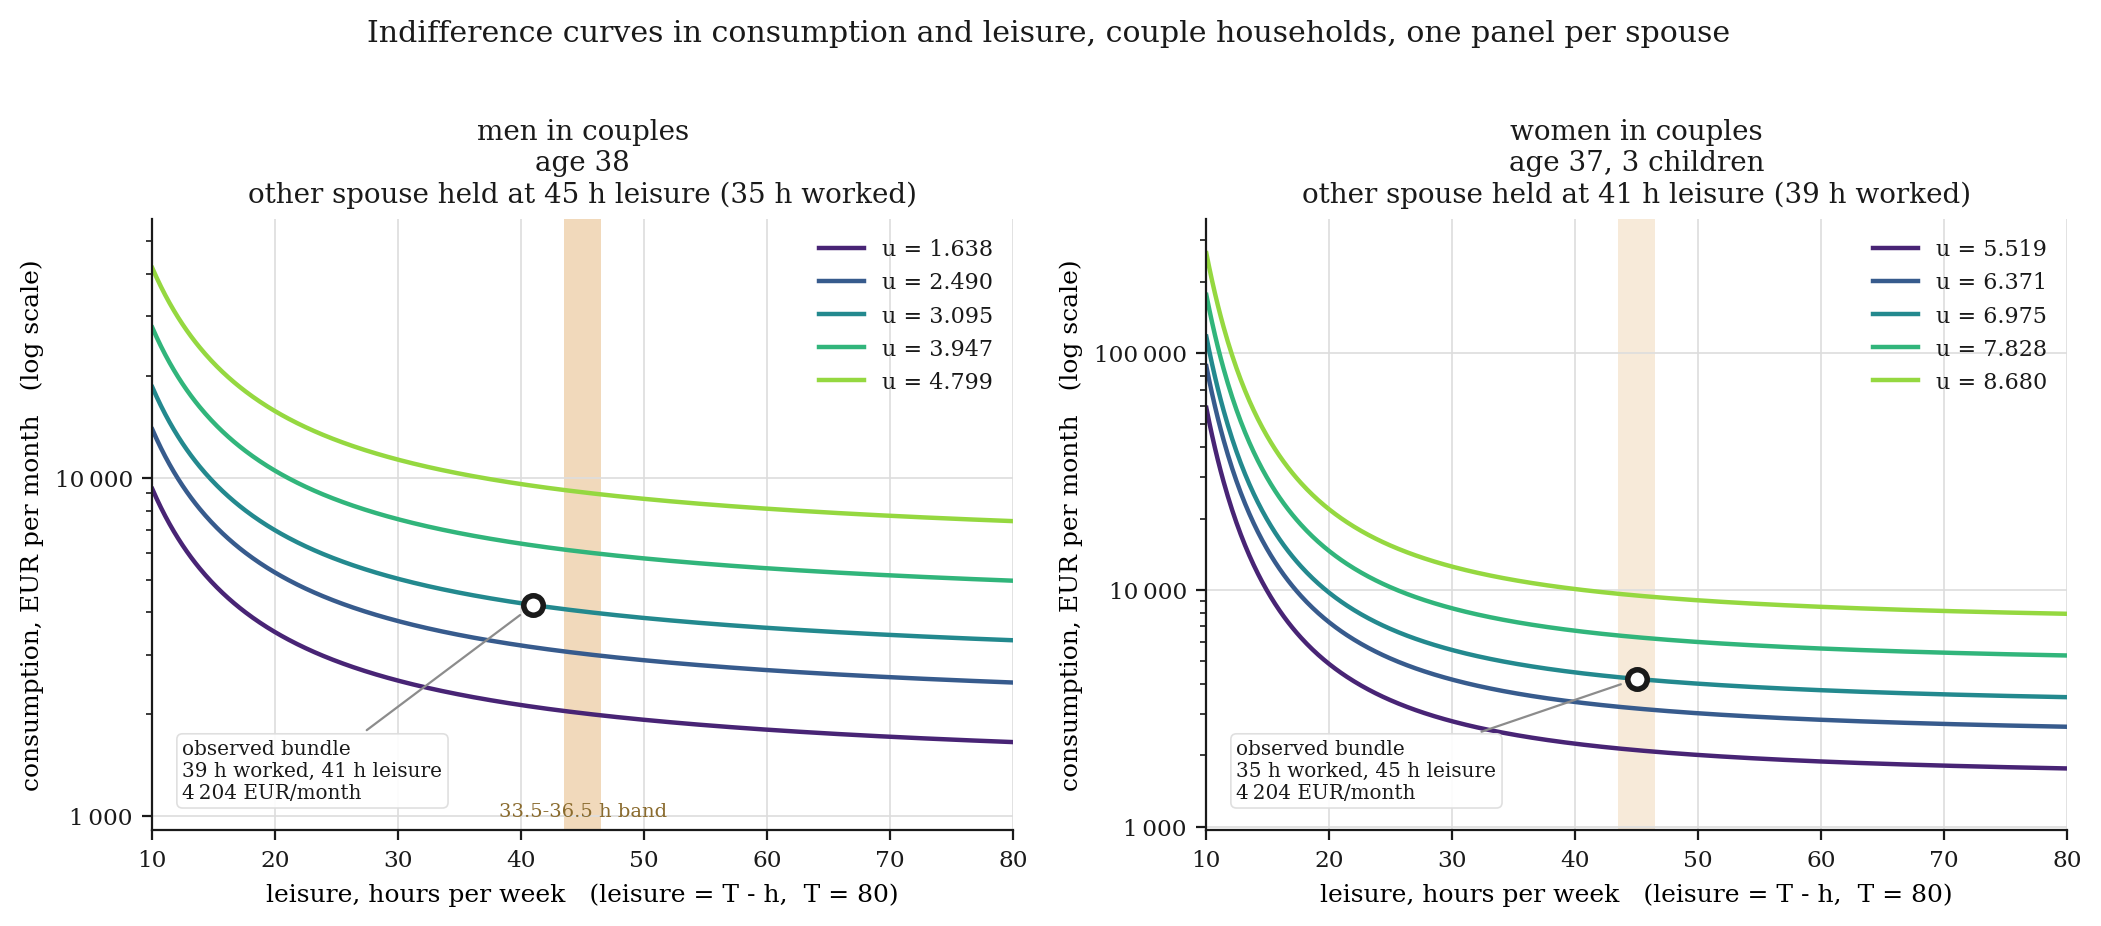
\includegraphics[width=0.95\linewidth,height=\textheight,keepaspectratio,alt={Indifference curves in consumption and each spouse's leisure, couple households, with the partner's leisure held at its observed value. Conditional slices of a joint object, not attainable sets.}]{figures/v5/figP02_indifference_curves_couples.png}
\caption{Indifference curves in consumption and each spouse's leisure, couple households, with the partner's leisure held at its observed value. Conditional slices of a joint object, not attainable sets.}
\end{figure}

\begin{figure}[H]
\centering
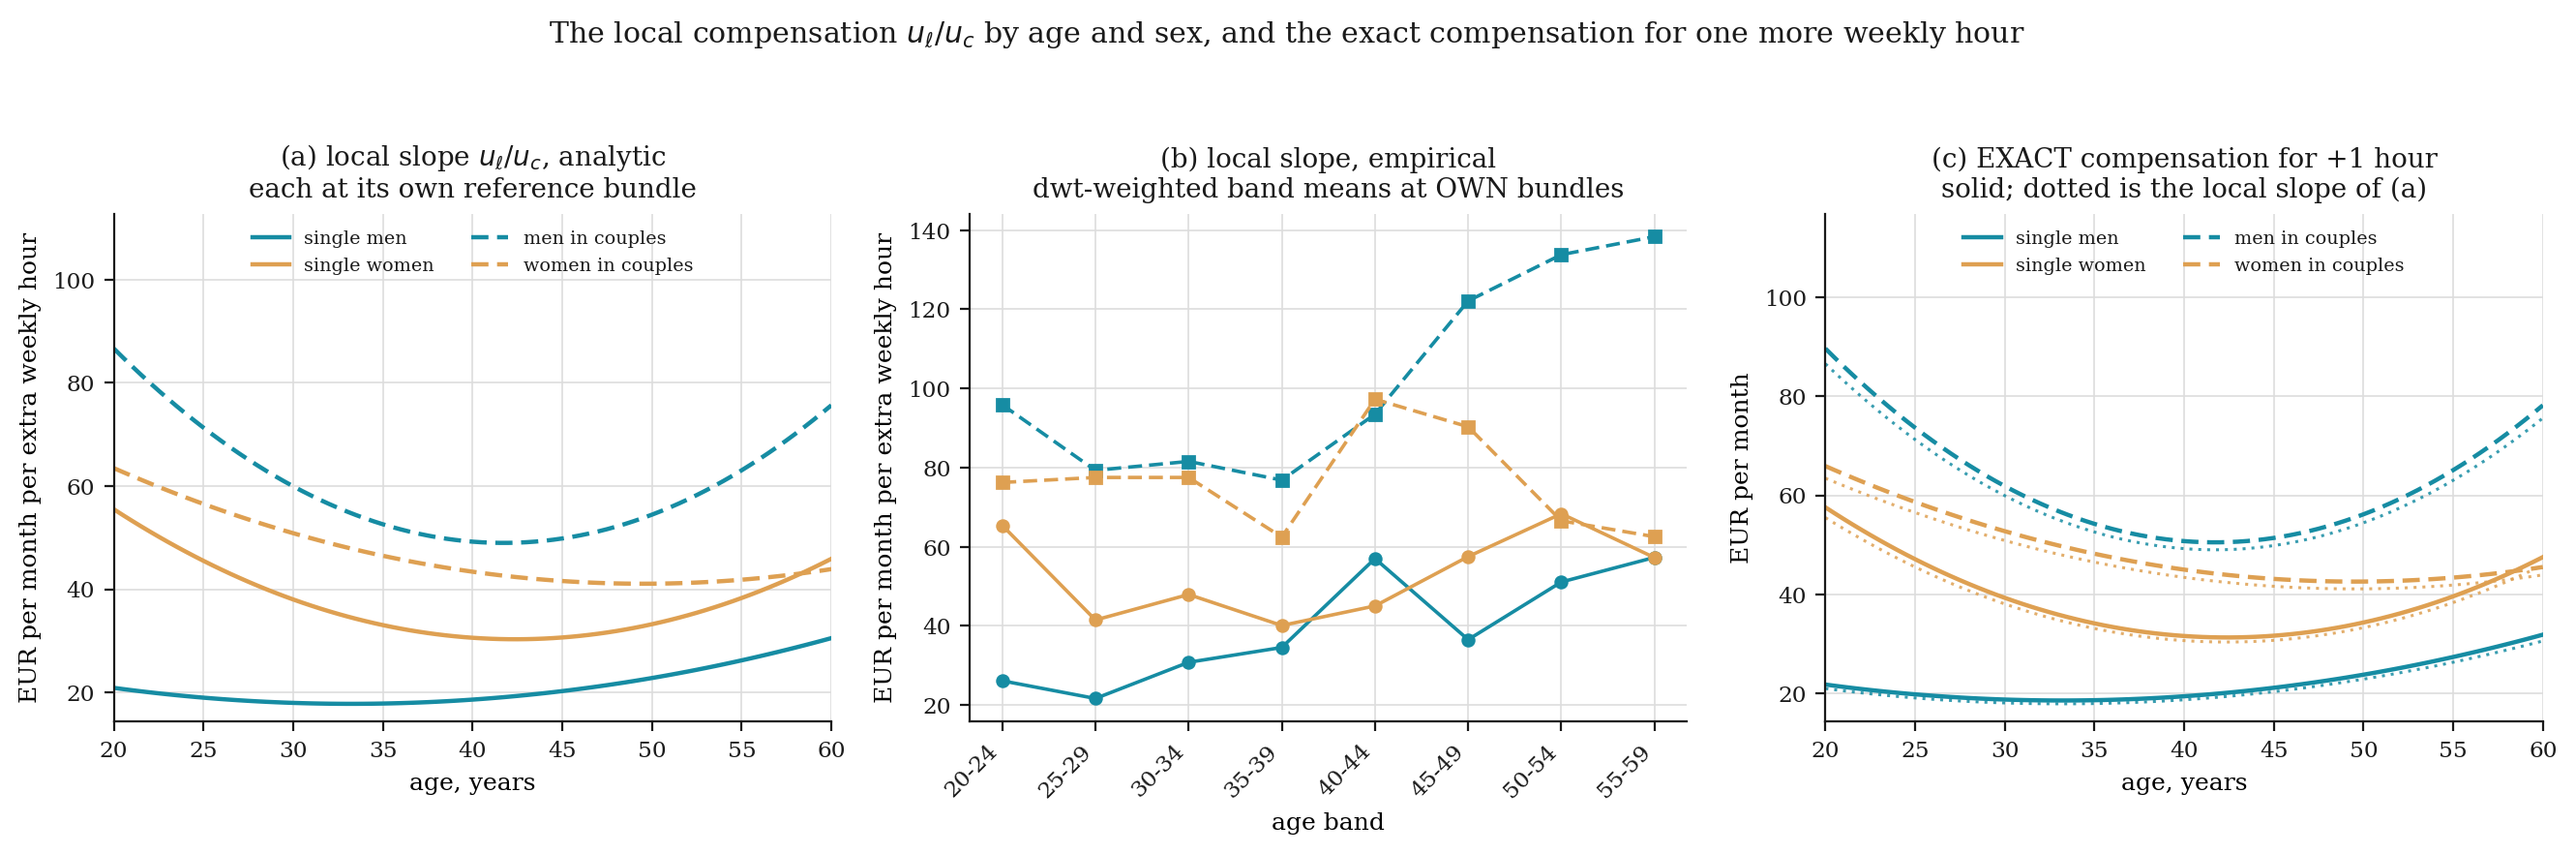
\includegraphics[width=0.95\linewidth,height=\textheight,keepaspectratio,alt={Marginal rate of substitution between leisure and consumption, by age and sex, in euros per month per additional recurring weekly hour of leisure. A compensation along an indifference curve, not a behavioural response to a wage change.}]{figures/v5/figP04_mrs_by_age_sex.png}
\caption{Marginal rate of substitution between leisure and consumption, by age and sex, in euros per month per additional recurring weekly hour of leisure. A compensation along an indifference curve, not a behavioural response to a wage change.}
\end{figure}

The indifference curves and the marginal rate of substitution are the economics; the coefficients are coordinates. Note that the consumption axis is logarithmic and the curves are drawn over the plotted range only: under \(L(\ell)+\beta_c\log(C/\lambda_c)\), any finite utility target at positive leisure is reached at the finite positive consumption \(C=\lambda_c\exp\{(\bar u-L(\ell))/\beta_c\}\), which is strictly positive for every finite target. A curve leaving the frame has left the plotting range, not the domain of the model, and nothing here is economically infeasible.

